\section*{Problem 5}

Consider the following directed graph for $n \geq 3$:

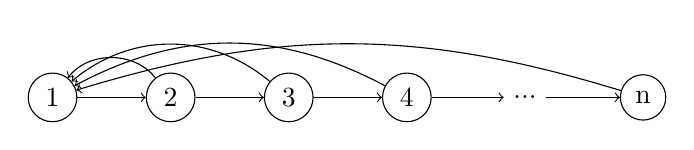
\begin{tikzpicture}
    \node[shape=circle,draw=black] (1) at (0,0) {1};
    \node[shape=circle,draw=black] (2) at (1.5,0) {2};
    \node[shape=circle,draw=black] (3) at (3,0) {3};
    \node[shape=circle,draw=black] (4) at (4.5,0) {4};
    \node (i) at (6,0) {...};
    \node[shape=circle,draw=black] (n) at (7.5,0) {n} ;

    \path [->](1) edge node [left] {}(2);
    \path [->](2) edge node [left] {}(3);
    \path [->](3) edge node [left] {}(4);
    \path [->](4) edge node [left] {}(i);
    \path [->](i) edge node [left] {}(n);
    
    \path [->](2) edge [bend right=52] node [right] {}(1);
    \path [->](3) edge [bend right=40] node [right] {}(1);
    \path [->](4) edge [bend right=28] node [right] {}(1);
    \path [->](n) edge [bend right=17] node [right] {}(1);

\end{tikzpicture}

This graph has a the directed edges $(i, i+1)$ and $(i+1, 1)$ for $1 \leq i < n$.

Thus, the graph has the a transition matrix $P \in [0, 1]^{n \times n}$ with the following entries:

$p_{1,2} = 1$,
$p_{n,1} = 1$

For $2 \leq i < n$: $p_{i, i + 1} = 0.5$ and $p_{i, 1} = 0.5$ 

For all other elements: $p_{i,j} = 0$.

Since the graph is irreducible (strongly connected) and aperiodic (there exits a path of length $n + 2$ and one of length $n + 3$ for every node and $\operatorname{gcd}(n + 2, n + 3) = 1$). Therefore, a unique stationary solution $\pi$ exists . By definition of a stationary solution, the following equation holds:

$\pi = \pi P$

Furthermore, by matrix multiplication we know for $j \in [1..n]$:

$\pi_j = \sum\limits_{i = 1}^n \pi_i \cdot p_{i,j}$

This yields the following linear equations for the given transition matrix $P$:

\begin{enumerate}[I:]
    \item $\pi_1 = \pi_n + 0.5 \cdot \sum\limits_{i = 2}^{n - 1} \pi_i$
    \item $\pi_2 = \pi_1$
    \item For $2 \leq i < n$: $\pi_{i + 1} = 0.5 \cdot \pi_i \Leftrightarrow 2 \cdot \pi_{i + 1} = \pi_{i}$ 
\end{enumerate}

\underline{Claim:} For $n \geq 3$: $2^{n-2}\cdot\pi_n = \pi_2$ 

\underline{Proof:} By induction on $n$, using equation III

Let $n \geq 3$ be arbitrary.

Case $n = 3$: $2^{3-2}\cdot\pi_3 = 2\cdot\pi_3 = \pi_2$

Case $n > 3$: $2^{n-2}\cdot\pi_n = 2^{n-3}\cdot(2 \cdot \pi_n) = 2^{n-3}\cdot(\pi_{n - 1}) = 2^{(n-1)-2}\cdot\pi_{n - 1} = \pi_2$

Therefore, for this graph and $u = 2, v = n$ the following holds:

$\frac{\pi_u}{\pi_v} = \frac{\pi_2}{\pi_n} = \frac{2^{n - 2} \cdot \pi_n}{\pi_n} = 2^{n - 2}$

Thus, $\pi_u/\pi_v = 2^{\Omega(n)}$.